\documentclass[a4paper,11pt]{ltjsarticle}
\usepackage{luatexja}
\usepackage{amsmath,amssymb,amsthm}
\usepackage{tikz-cd}
\usepackage{tikz}
\usetikzlibrary{positioning,arrows.meta,shapes.geometric}
\usepackage{hyperref}
\usepackage{listings}
\usepackage{xcolor}

% 定理環境
\theoremstyle{definition}
\newtheorem{definition}{定義}[section]
\newtheorem{theorem}[definition]{定理}
\newtheorem{lemma}[definition]{補題}
\newtheorem{proposition}[definition]{命題}
\newtheorem{example}[definition]{例}
\newtheorem{remark}[definition]{注意}

% Leanコード用の設定
\lstdefinelanguage{Lean}{
  morekeywords={def,theorem,lemma,structure,where,by,intro,exact,have,constructor,refine,simp,funext,ext,noncomputable,variable,section,end,namespace,open,example},
  sensitive=true,
  morecomment=[l]{--},
  morecomment=[s]{/-}{-/},
  morestring=[b]",
}

\lstset{
  language=Lean,
  basicstyle=\ttfamily\small,
  keywordstyle=\color{blue}\bfseries,
  commentstyle=\color{green!60!black},
  stringstyle=\color{red},
  showstringspaces=false,
  breaklines=true,
  frame=single,
  numbers=left,
  numberstyle=\tiny\color{gray},
}

\title{Rank関数と構造塔の正準対応\\
{\large RankTower.leanの数学的解説}}
\author{%
Leanコード生成：CODEX (OpenAI)\\
\LaTeX 文書作成：Claude Code (Anthropic)%
}
\date{\today}

\begin{document}

\maketitle

\begin{abstract}
本稿では、Lean 4で実装された構造塔（Structure Tower）とランク関数（Rank Function）の双方向対応について数学的に詳細な解説を行う。この対応により、階層的構造を持つ数学的対象を統一的に扱うことが可能となり、「階層＝ランク」という正規形が得られる。具体的な応用例として、有理ベクトル空間における線形従属性の階層構造（Vec2Q）や、自然数の順序構造、有限集合の濃度などを示す。
\end{abstract}

\tableofcontents

\section{導入}

\subsection{動機}

数学において、対象を階層的に分類することは基本的な手法である：
\begin{itemize}
\item トポロジーにおける次元（0次元＝点、1次元＝曲線、2次元＝曲面、…）
\item 代数学におけるランク（ベクトル空間の次元、加群のランク、…）
\item 集合論における濃度（有限集合の要素数）
\item 確率論における停止時間（フィルトレーションの階層）
\end{itemize}

これらの概念を統一的に扱うために、本稿では以下の双方向対応を確立する：

\[
\boxed{\text{構造塔（StructureTowerWithMin）} \;\leftrightarrow\; \text{ランク関数（} X \to \mathbb{N} \cup \{\top\} \text{）}}
\]

\subsection{主要結果の概要}

\begin{theorem}[正規形定理]\label{thm:main}
以下の対応が成立する：
\begin{enumerate}
\item 任意のランク関数 $\rho : X \to \mathbb{N} \cup \{\top\}$（被覆条件を満たす）から構造塔を構成できる。
\item 任意の構造塔 $T$ からランク関数 $\rho_T$ を抽出できる。
\item これらの構成は互いに逆である：
\begin{itemize}
\item $\rho \mapsto T_\rho \mapsto \rho_{T_\rho} = \rho$（ランク関数の往復）
\item $T \mapsto \rho_T \mapsto T_{\rho_T} \cong T$（構造塔の往復、層ごとの同型）
\end{itemize}
\end{enumerate}
\end{theorem}

\section{基本定義}

\subsection{構造塔}

\begin{definition}[最小層を持つ構造塔]\label{def:tower}
構造塔 $T$ は以下のデータからなる：
\begin{itemize}
\item 台集合 $X$（carrier）
\item 層の族 $\{\ell_n\}_{n \in \mathbb{N}}$（layer $: \mathbb{N} \to \mathcal{P}(X)$）
\item 被覆性：$\forall x \in X, \exists n \in \mathbb{N}, x \in \ell_n$
\item 単調性：$i \leq j \Rightarrow \ell_i \subseteq \ell_j$
\item 最小層関数：$\mathrm{minLayer} : X \to \mathbb{N}$
\item 最小層の性質：
\begin{itemize}
\item $\forall x, x \in \ell_{\mathrm{minLayer}(x)}$（所属性）
\item $\forall x, i, (x \in \ell_i \Rightarrow \mathrm{minLayer}(x) \leq i)$（最小性）
\end{itemize}
\end{itemize}
\end{definition}

\begin{remark}
最小層 $\mathrm{minLayer}(x)$ は、$x$ が初めて現れる層の番号である。単調性により、$x \in \ell_n$ ならば $x \in \ell_m$ for all $m \geq n$ が成り立つ。
\end{remark}

\subsection{ランク関数}

\begin{definition}[ランク関数]\label{def:rank}
集合 $X$ 上のランク関数とは、写像
\[
\rho : X \to \mathbb{N} \cup \{\top\}
\]
であり、以下の被覆条件を満たすもの：
\[
\forall x \in X, \exists n \in \mathbb{N}, \rho(x) \leq n
\]
ここで $\top$ は「無限大」を表す要素である（WithTop $\mathbb{N}$）。
\end{definition}

\begin{remark}
被覆条件は、$\rho(x) = \top$ となる $x$ が存在しないことを保証する。実用上は、$\rho : X \to \mathbb{N}$ としても差し支えない。
\end{remark}

\section{順方向の構成：ランク関数から構造塔へ}

\subsection{構成}

\begin{definition}[ランク関数から誘導される構造塔]\label{def:rank_to_tower}
ランク関数 $\rho : X \to \mathbb{N} \cup \{\top\}$ が被覆条件を満たすとき、構造塔 $T_\rho$ を以下で定義する：
\begin{align*}
\text{台集合：} & \quad X \\
\text{層：} & \quad \ell_n := \{x \in X \mid \rho(x) \leq n\} \\
\text{最小層：} & \quad \mathrm{minLayer}(x) := \min\{n \in \mathbb{N} \mid \rho(x) \leq n\}
\end{align*}
\end{definition}

\begin{proposition}[構造塔の公理の充足]\label{prop:rank_gives_tower}
定義\ref{def:rank_to_tower}の $T_\rho$ は、定義\ref{def:tower}の構造塔の公理を満たす。
\end{proposition}

\begin{proof}[証明の概略]
\begin{itemize}
\item \textbf{被覆性}：$\rho$ の被覆条件より、各 $x$ に対して $\rho(x) \leq n$ なる $n$ が存在するので、$x \in \ell_n$。
\item \textbf{単調性}：$i \leq j$ のとき、$\rho(x) \leq i \Rightarrow \rho(x) \leq j$ より $\ell_i \subseteq \ell_j$。
\item \textbf{最小層の所属性}：$\mathrm{minLayer}(x)$ の定義より、$\rho(x) \leq \mathrm{minLayer}(x)$ が成り立つので $x \in \ell_{\mathrm{minLayer}(x)}$。
\item \textbf{最小層の最小性}：$x \in \ell_i$ ならば $\rho(x) \leq i$ なので、$\mathrm{minLayer}(x) \leq i$。
\end{itemize}
\end{proof}

\subsection{ランク関数が自然数値の場合の特別な性質}

\begin{lemma}[最小層とランクの一致]\label{lem:minlayer_eq_rank}
$\rho : X \to \mathbb{N}$ が自然数値のランク関数のとき、
\[
\mathrm{minLayer}_{T_\rho}(x) = \rho(x)
\]
が成り立つ。
\end{lemma}

\begin{proof}
$\mathrm{minLayer}(x) := \min\{n \mid \rho(x) \leq n\}$ であり、$\rho(x) \in \mathbb{N}$ なので、$n = \rho(x)$ が条件を満たす最小の値である。したがって $\mathrm{minLayer}(x) = \rho(x)$。
\end{proof}

\section{逆方向の構成：構造塔からランク関数へ}

\subsection{構成}

\begin{definition}[構造塔から誘導されるランク関数]\label{def:tower_to_rank}
構造塔 $T$ に対して、ランク関数 $\rho_T : X \to \mathbb{N} \cup \{\top\}$ を
\[
\rho_T(x) := \mathrm{minLayer}_T(x)
\]
で定義する（自然数を $\mathbb{N} \cup \{\top\}$ に埋め込む）。
\end{definition}

\begin{proposition}[ランク関数の性質]\label{prop:tower_gives_rank}
定義\ref{def:tower_to_rank}の $\rho_T$ はランク関数の被覆条件を満たす。
\end{proposition}

\begin{proof}
各 $x \in X$ に対して、$\mathrm{minLayer}_T(x) \in \mathbb{N}$ なので、$n := \mathrm{minLayer}_T(x)$ とおけば $\rho_T(x) = n \leq n$。
\end{proof}

\subsection{ランクと層の特徴付け}

\begin{lemma}[ランクと層の同値性]\label{lem:rank_layer_equiv}
構造塔 $T$ から誘導されるランク関数 $\rho_T$ について、
\[
\rho_T(x) \leq n \quad\Leftrightarrow\quad x \in \ell_n
\]
が成り立つ。
\end{lemma}

\begin{proof}
\begin{description}
\item[($\Rightarrow$)] $\rho_T(x) \leq n$ すなわち $\mathrm{minLayer}(x) \leq n$ とする。最小層の所属性より $x \in \ell_{\mathrm{minLayer}(x)}$ であり、単調性より $x \in \ell_n$。
\item[($\Leftarrow$)] $x \in \ell_n$ とする。最小層の最小性より $\mathrm{minLayer}(x) \leq n$、すなわち $\rho_T(x) \leq n$。
\end{description}
\end{proof}

\section{双方向対応の証明}

\subsection{順方向の往復}

\begin{theorem}[ランク関数の往復同型]\label{thm:rank_roundtrip}
$\rho : X \to \mathbb{N}$ を自然数値のランク関数とする。このとき、
\[
\rho_{T_\rho} = \rho
\]
すなわち、$\rho$ から構造塔 $T_\rho$ を作り、そこからランク関数を抽出すると元の $\rho$ に戻る。
\end{theorem}

\begin{proof}
定義より、
\[
\rho_{T_\rho}(x) = \mathrm{minLayer}_{T_\rho}(x) = \rho(x)
\]
最後の等号は補題\ref{lem:minlayer_eq_rank}による。
\end{proof}

\subsection{逆方向の往復}

\begin{theorem}[構造塔の往復同型]\label{thm:tower_roundtrip}
構造塔 $T$ に対して、$T_{\rho_T}$ と $T$ は層ごとに一致する：
\[
\forall n \in \mathbb{N}, \quad \ell^{T_{\rho_T}}_n = \ell^T_n
\]
\end{theorem}

\begin{proof}
定義より、
\begin{align*}
x \in \ell^{T_{\rho_T}}_n
&\Leftrightarrow \rho_T(x) \leq n \\
&\Leftrightarrow \mathrm{minLayer}_T(x) \leq n \\
&\Leftrightarrow x \in \ell^T_n
\end{align*}
最後の同値は補題\ref{lem:rank_layer_equiv}による。
\end{proof}

\subsection{図式による対応の表現}

この双方向対応は以下の図式で表現できる：

\begin{center}
\begin{tikzcd}[row sep=huge, column sep=huge]
\text{ランク関数} \arrow[r, bend left=30, "\text{層構成}"] \arrow[loop left, "\text{id}"]
& \text{構造塔} \arrow[l, bend left=30, "\text{minLayer}"] \arrow[loop right, "\cong"]
\end{tikzcd}
\end{center}

より詳細には：

\begin{center}
\begin{tikzcd}[row sep=large, column sep=large]
\rho : X \to \mathbb{N} \arrow[r, mapsto] \arrow[d, phantom, "="]
& T_\rho \arrow[r, mapsto]
& \rho_{T_\rho} \arrow[d, phantom, "="] \\
\rho
& \ell_n = \{x \mid \rho(x) \leq n\}
& \rho
\end{tikzcd}
\end{center}

\section{具体例}

\subsection{有理ベクトル空間における線形従属性（Vec2Q）}

\begin{example}[2次元有理ベクトルの最小基底数]\label{ex:vec2q}
$V := \mathbb{Q}^2$ とし、ベクトル $v = (v_1, v_2) \in V$ に対して、
\[
\rho(v) := \mathrm{minBasisCount}(v) := \begin{cases}
0 & \text{if } v = (0, 0) \\
1 & \text{if } v \neq (0,0) \text{ かつ } v_1 = 0 \text{ または } v_2 = 0 \\
2 & \text{otherwise}
\end{cases}
\]
と定義する。これはランク関数であり、誘導される構造塔は：
\begin{align*}
\ell_0 &= \{(0, 0)\} \quad\text{（零ベクトル）} \\
\ell_1 &= \{(0, 0)\} \cup \{(v_1, 0) \mid v_1 \neq 0\} \cup \{(0, v_2) \mid v_2 \neq 0\} \quad\text{（1次元部分空間）} \\
\ell_2 &= \mathbb{Q}^2 \quad\text{（全体）}
\end{align*}
\end{example}

この例の階層構造を図示すると：

\begin{center}
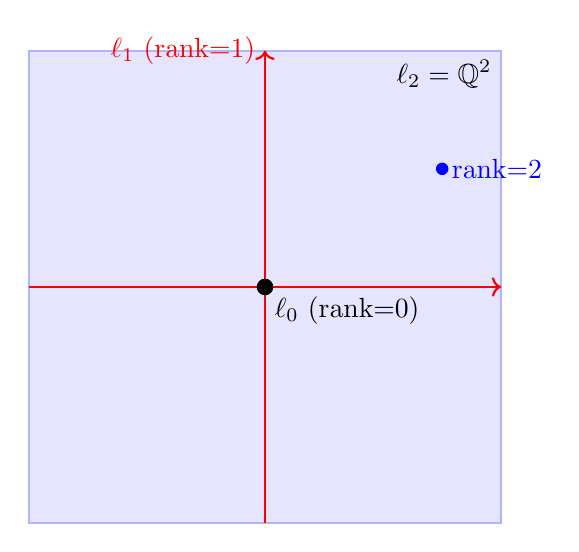
\begin{tikzpicture}[scale=1.5]
% 層2（全体）
\draw[thick, blue!30, fill=blue!10] (-2,-2) rectangle (2,2);
\node[anchor=north east] at (2,2) {$\ell_2 = \mathbb{Q}^2$};

% 層1（座標軸）
\draw[thick, red, ->] (-2,0) -- (2,0);
\draw[thick, red, ->] (0,-2) -- (0,2);
\node[anchor=east, red] at (0,2) {$\ell_1$ (rank=1)};

% 層0（原点）
\fill[black] (0,0) circle (2pt);
\node[anchor=north west] at (0,0) {$\ell_0$ (rank=0)};

% 一般点の例
\fill[blue] (1.5,1) circle (1.5pt);
\node[anchor=west, blue] at (1.5,1) {rank=2};
\end{tikzpicture}
\end{center}

\begin{remark}
この例は、ベクトルを「生成に必要な最小基底の数」で階層化する。これは線形代数におけるランクの概念と整合的である。
\end{remark}

\subsection{自然数の恒等ランク}

\begin{example}[自然数の順序構造]\label{ex:nat_rank}
$\rho : \mathbb{N} \to \mathbb{N}$ を恒等写像 $\rho(n) = n$ とする。誘導される構造塔は：
\[
\ell_n = \{k \in \mathbb{N} \mid k \leq n\} = \{0, 1, 2, \ldots, n\}
\]
すなわち、自然数の通常の順序構造を表現する。
\end{example}

\begin{center}
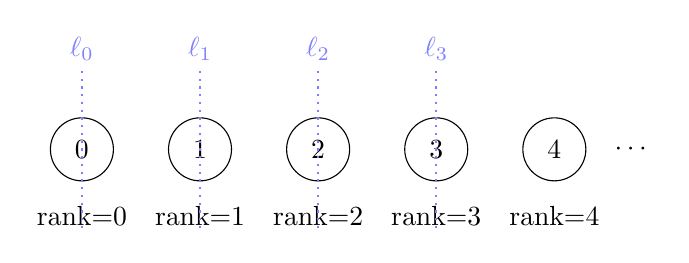
\begin{tikzpicture}
\foreach \n in {0,1,2,3,4} {
  \node[circle, draw, minimum size=0.8cm] (n\n) at (\n*1.5,0) {$\n$};
  \node[below] at (\n*1.5,-0.6) {rank=$\n$};
}
\draw[thick, blue!50, dotted] (0,-1) -- (0,1) node[above] {$\ell_0$};
\draw[thick, blue!50, dotted] (1.5,-1) -- (1.5,1) node[above] {$\ell_1$};
\draw[thick, blue!50, dotted] (3,-1) -- (3,1) node[above] {$\ell_2$};
\draw[thick, blue!50, dotted] (4.5,-1) -- (4.5,1) node[above] {$\ell_3$};
\node at (7,0) {$\cdots$};
\end{tikzpicture}
\end{center}

\subsection{有限集合の濃度}

\begin{example}[部分集合の濃度ランク]\label{ex:cardinality}
$n \in \mathbb{N}$ を固定し、$X := \mathcal{P}(\{1, 2, \ldots, n\})$（冪集合）とする。
\[
\rho(S) := |S| \quad\text{（集合 } S \text{ の濃度）}
\]
と定義すると、誘導される構造塔は：
\[
\ell_k = \{S \subseteq \{1, \ldots, n\} \mid |S| \leq k\}
\]
特に、$\ell_0 = \{\emptyset\}$、$\ell_n = \mathcal{P}(\{1, \ldots, n\})$ である。
\end{example}

$n=3$ の場合の例：

\begin{center}
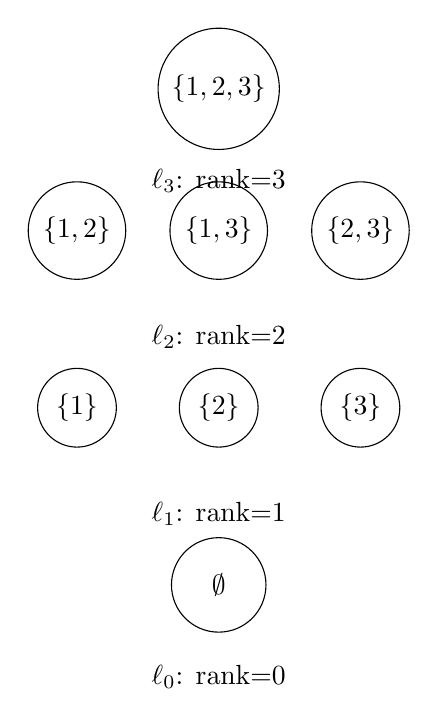
\begin{tikzpicture}[scale=0.9]
% 層0
\node[draw, circle, minimum size=1.2cm] (empty) at (0,0) {$\emptyset$};
\node[below] at (0,-1) {$\ell_0$: rank=0};

% 層1
\node[draw, circle, minimum size=1cm] (s1) at (-2,2.5) {$\{1\}$};
\node[draw, circle, minimum size=1cm] (s2) at (0,2.5) {$\{2\}$};
\node[draw, circle, minimum size=1cm] (s3) at (2,2.5) {$\{3\}$};
\node[below] at (0,1.3) {$\ell_1$: rank=1};

% 層2
\node[draw, circle, minimum size=0.9cm] (s12) at (-2,5) {$\{1,2\}$};
\node[draw, circle, minimum size=0.9cm] (s13) at (0,5) {$\{1,3\}$};
\node[draw, circle, minimum size=0.9cm] (s23) at (2,5) {$\{2,3\}$};
\node[below] at (0,3.8) {$\ell_2$: rank=2};

% 層3
\node[draw, circle, minimum size=0.9cm] (full) at (0,7) {$\{1,2,3\}$};
\node[below] at (0,6) {$\ell_3$: rank=3};
\end{tikzpicture}
\end{center}

\section{理論的意義と応用}

\subsection{概念の統一}

定理\ref{thm:main}により、以下の概念が統一的に理解できる：

\begin{center}
\begin{tikzpicture}[
  box/.style={rectangle, draw, minimum width=3cm, minimum height=1cm, text centered, rounded corners},
  arrow/.style={-Stealth, thick}
]
\node[box] (rank) at (0,0) {ランク関数};
\node[box] (tower) at (6,0) {構造塔};

\node[box, fill=blue!10] (dim) at (-3,-2.5) {次元理論};
\node[box, fill=green!10] (order) at (0,-2.5) {順序理論};
\node[box, fill=red!10] (card) at (3,-2.5) {濃度理論};
\node[box, fill=yellow!10] (stop) at (6,-2.5) {停止時間};

\draw[arrow, <->] (rank) -- (tower);
\draw[arrow] (dim) -- (rank);
\draw[arrow] (order) -- (rank);
\draw[arrow] (card) -- (tower);
\draw[arrow] (stop) -- (tower);
\end{tikzpicture}
\end{center}

\subsection{確率論への応用：停止時間}

停止時間 $\tau : \Omega \to \mathbb{N}$（確率空間 $\Omega$ 上）は、まさにランク関数である：
\begin{itemize}
\item $\rho(x) = \tau(x)$：標本点 $x$ での停止時刻
\item $\ell_n = \{x \in \Omega \mid \tau(x) \leq n\}$：時刻 $n$ までに停止する集合
\end{itemize}

フィルトレーション $(\mathcal{F}_n)_{n \geq 0}$ との関係：
\[
\{x \mid \tau(x) \leq n\} \in \mathcal{F}_n \quad\text{（可測性）}
\]
は、構造塔の単調性に対応する。

\subsection{代数への応用：加群のランク}

自由加群 $M = R^n$ において、部分加群 $N \subseteq M$ のランク $\rho(N)$ は：
\[
\rho(N) := \text{生成元の最小個数}
\]
これは構造塔を誘導し、部分加群の階層を記述する。

\section{Lean 4実装の概要}

\subsection{主要な定義}

Leanでの実装では、WithTop型（$\mathbb{N} \cup \{\top\}$）を用いて無限大を表現する：

\begin{lstlisting}
structure StructureTowerWithMin where
  carrier : Type*
  layer : ℕ → Set carrier
  covering : ∀ x : carrier, ∃ i : ℕ, x ∈ layer i
  monotone : ∀ {i j : ℕ}, i ≤ j → layer i ⊆ layer j
  minLayer : carrier → ℕ
  minLayer_mem : ∀ x, x ∈ layer (minLayer x)
  minLayer_minimal : ∀ x i, x ∈ layer i → minLayer x ≤ i
\end{lstlisting}

\subsection{順方向構成の実装}

\begin{lstlisting}
noncomputable def towerFromRank (ρ : X → WithTop ℕ)
    (h_covers : ∀ x, ∃ n : ℕ, ρ x ≤ n) :
    StructureTowerWithMin where
  carrier := X
  layer n := {x : X | ρ x ≤ n}
  minLayer := fun x => Nat.find (h_covers x)
  -- ... (証明は省略)
\end{lstlisting}

ここで \texttt{Nat.find} は、述語を満たす最小の自然数を返す非計算的関数である。

\subsection{往復同型の証明}

\begin{lstlisting}
theorem rankFromTower_towerFromRank (ρ : X → ℕ)
    (h : ∀ x, ∃ n : ℕ, (ρ x : WithTop ℕ) ≤ n) (x : X) :
    rankFromTower (towerFromRank (fun x => (ρ x : WithTop ℕ)) h) x = ρ x := by
  have hmin := towerFromRank_minLayer_eq_rank (ρ := ρ) h x
  simp [rankFromTower, hmin]
\end{lstlisting}

この証明は、補題\ref{lem:minlayer_eq_rank}に相当する \texttt{towerFromRank\_minLayer\_eq\_rank} を用いて、単純化（\texttt{simp}）により完了する。

\section{今後の展望}

\subsection{連続版への拡張}

離散的な階層（$\mathbb{N}$）から連続的な階層（$\mathbb{R}_{\geq 0}$）への拡張：
\[
\rho : X \to \mathbb{R}_{\geq 0} \cup \{\infty\}
\]
これにより、連続時間の停止時間や、フラクタル次元などを扱える。

\subsection{圏論的定式化}

構造塔とランク関数の対応を、圏同値として定式化：
\[
\mathbf{Tower} \simeq \mathbf{RankFunc}
\]
関手の構成と自然同型の証明が今後の課題である。

\subsection{Optional Stopping Theoremとの統合}

確率論における Optional Stopping Theorem（OST）を、Rank型構造塔の普遍性から導出する試みが進行中である。これにより、マルチンゲール理論と構造塔理論の深い関係が明らかになると期待される。

\section{結論}

本稿では、Lean 4で形式化された「ランク関数と構造塔の双方向対応」について、数学的に詳細な解説を行った。この対応により：

\begin{itemize}
\item 階層的構造を持つ様々な数学的対象が統一的に扱える
\item 「階層＝ランク」という明快な正規形が得られる
\item 具体的な応用（ベクトル空間、順序集合、確率論など）が豊富に存在する
\item Lean 4での形式的証明により、理論の厳密性が保証される
\end{itemize}

今後は、連続版への拡張や圏論的定式化、確率論との更なる統合が期待される。

\appendix

\section{記号表}

\begin{tabular}{ll}
$X$ & 台集合（carrier） \\
$\rho$ & ランク関数（rank function） \\
$T$ & 構造塔（structure tower） \\
$\ell_n$ & 第 $n$ 層（layer） \\
$\mathrm{minLayer}(x)$ & 要素 $x$ の最小層 \\
$\mathbb{N} \cup \{\top\}$ & WithTop $\mathbb{N}$（自然数に無限大を追加） \\
$\mathcal{P}(S)$ & 集合 $S$ の冪集合 \\
$\Omega$ & 確率空間の標本空間 \\
$\mathcal{F}_n$ & フィルトレーションの第 $n$ シグマ代数 \\
\end{tabular}

\section{参考文献}

\begin{itemize}
\item Bourbaki, N. \textit{Elements of Mathematics: Theory of Sets}. Springer.
\item Williams, D. \textit{Probability with Martingales}. Cambridge University Press.
\item Lean 4 Documentation: \url{https://leanprover.github.io/lean4/doc/}
\item Mathlib Documentation: \url{https://leanprover-community.github.io/mathlib4_docs/}
\end{itemize}

\end{document}
